% IEEE Double-Column Template with Appendix
% Compile: pdflatex -> bibtex -> pdflatex -> pdflatex

\documentclass[conference]{IEEEtran}
\IEEEoverridecommandlockouts

\usepackage[numbers]{natbib}
\usepackage{amsmath,amssymb,amsfonts}
\usepackage{algorithm}
\usepackage{algorithmic}
\usepackage{graphicx}
\usepackage{textcomp}
\usepackage{xcolor}
\usepackage{url}
\usepackage{booktabs}
\usepackage{multirow}
\usepackage{listings}

\lstset{
  basicstyle=\ttfamily\small,
  breaklines=true,
  frame=single,
  captionpos=b
}

\begin{document}

\title{Player Churn Prediction Using Streamlit and Machine Learning Pipelines}

\author{
\IEEEauthorblockN{Atharv Paharia, Khyati Kapil}
\IEEEauthorblockA{Team Name: Player Churn Analytics}
}

\maketitle

\begin{abstract}
This project presents an end-to-end player churn prediction system built with Streamlit and classical machine learning models. The pipeline supports robust preprocessing, dynamic target handling, multi-model training, evaluation, feature-importance analysis, risk segmentation, and single-player inference. Three classifiers (Logistic Regression, Random Forest, and Decision Tree) are trained using a unified preprocessing pipeline with imputation, scaling, and one-hot encoding. The app produces standard metrics, confusion matrices, risk-probability distributions, and interpretable model drivers to support retention strategy decisions.
\end{abstract}

\begin{IEEEkeywords}
Player churn, machine learning, Streamlit, classification, feature engineering, model interpretability.
\end{IEEEkeywords}

\section{Introduction}
Player churn directly affects revenue, engagement, and long-term platform growth in online games and digital products. Early identification of high-risk players enables targeted intervention campaigns such as rewards, recommendations, and personalized engagement. The goal of this project is to build an interactive ML application that predicts player churn risk and provides interpretable insights for product and retention teams.

\section{Related Work}
Customer and player churn prediction is commonly modeled as supervised binary classification, using models such as Logistic Regression, tree-based methods, and ensemble approaches \cite{burez2009churn,verbeke2012new}. Prior work highlights the usefulness of behavioral features and interpretable outputs for operational decisions \cite{huang2012churn}. Our project follows this direction with a practical app-first implementation.

\section{Methodology}

\subsection{Dataset Description}
The dataset (\texttt{online\_gaming\_behavior\_dataset.csv}) contains 40,034 player records and 13 features, including demographics, game behavior, and progression signals. The target is \texttt{EngagementLevel}. For churn-style binary modeling, \texttt{Low} engagement is mapped as positive class (churn = 1), while other classes are mapped to non-churn (0).

\subsection{Preprocessing}
The preprocessing stack includes:
\begin{itemize}
    \item Median imputation + standard scaling for numeric features
    \item Most-frequent imputation + one-hot encoding for categorical features
    \item Optional removal of high-cardinality ID columns from model training
\end{itemize}
A \texttt{ColumnTransformer} ensures consistent preprocessing across all models.

\subsection{Feature Engineering}
An engagement feature is created when session frequency and average session duration are available:
\[
\texttt{engagement\_score} = \texttt{session\_frequency} \times \texttt{avg\_session\_duration}
\]
Risk buckets are defined from predicted churn probability:
Low ($\leq 0.30$), Medium ($0.30$--$0.70$), High ($>0.70$).

\subsection{Models Used}
The training module fits three classifiers:
\begin{itemize}
    \item Logistic Regression
    \item Random Forest
    \item Decision Tree
\end{itemize}
Class-weight balancing is enabled when class imbalance is detected.

\subsection{Training and Validation}
Data is split into train/test sets using an 80/20 split with fixed random seed (\texttt{random\_state=42}) and stratification. Evaluation includes Accuracy, Precision, Recall, F1-score, ROC-AUC, confusion matrix visualization, feature-importance plots, and risk distribution analysis.

\section{Results}

\subsection{Quantitative Results}
\begin{table}[ht]
\centering
\caption{Model Performance Comparison}
\begin{tabular}{lccccc}
\toprule
Model & Acc & Prec & Rec & F1 & ROC-AUC \\
\midrule
Logistic Regression & 0.840 & 0.634 & 0.897 & 0.743 & 0.926 \\
Random Forest & \textbf{0.950} & \textbf{0.914} & \textbf{0.890} & \textbf{0.902} & \textbf{0.938} \\
Decision Tree & 0.913 & 0.798 & 0.889 & 0.841 & 0.931 \\
\bottomrule
\end{tabular}
\label{tab:model_performance}
\end{table}

\subsection{Figures}
\begin{figure}[ht]
\centering
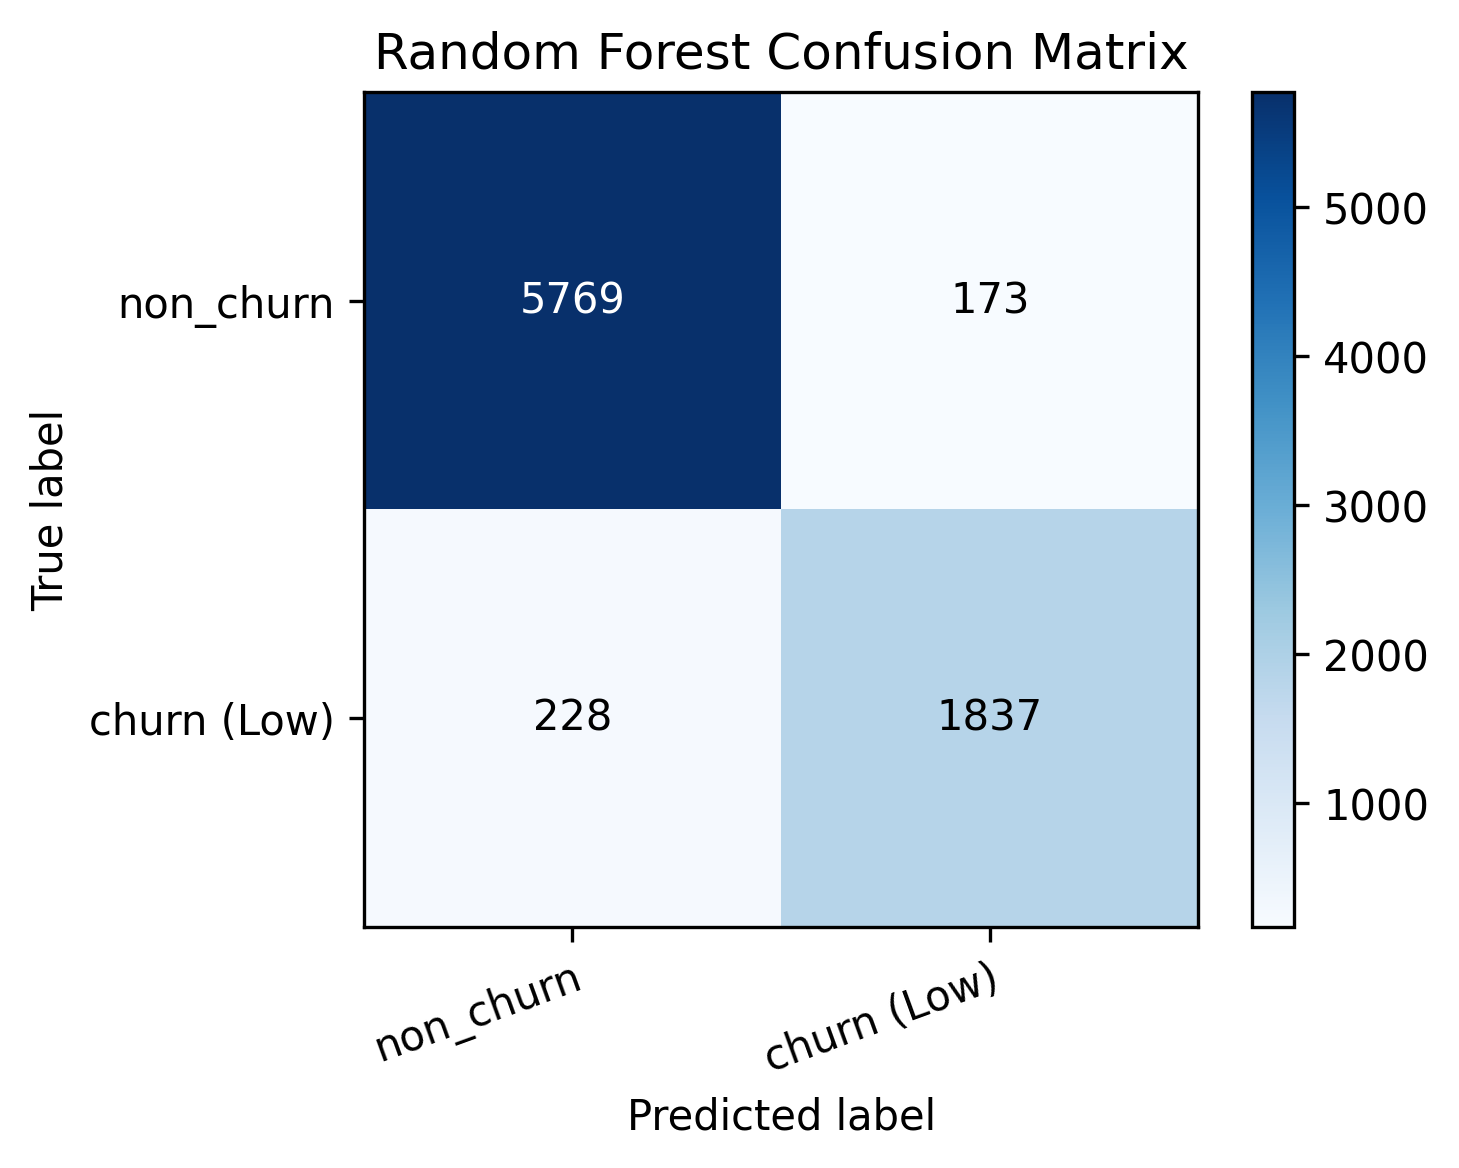
\includegraphics[width=0.45\textwidth]{figures/rf_confusion_matrix.png}
\caption{Random Forest confusion matrix on test data.}
\label{fig:rf_confusion}
\end{figure}

\begin{figure}[ht]
\centering
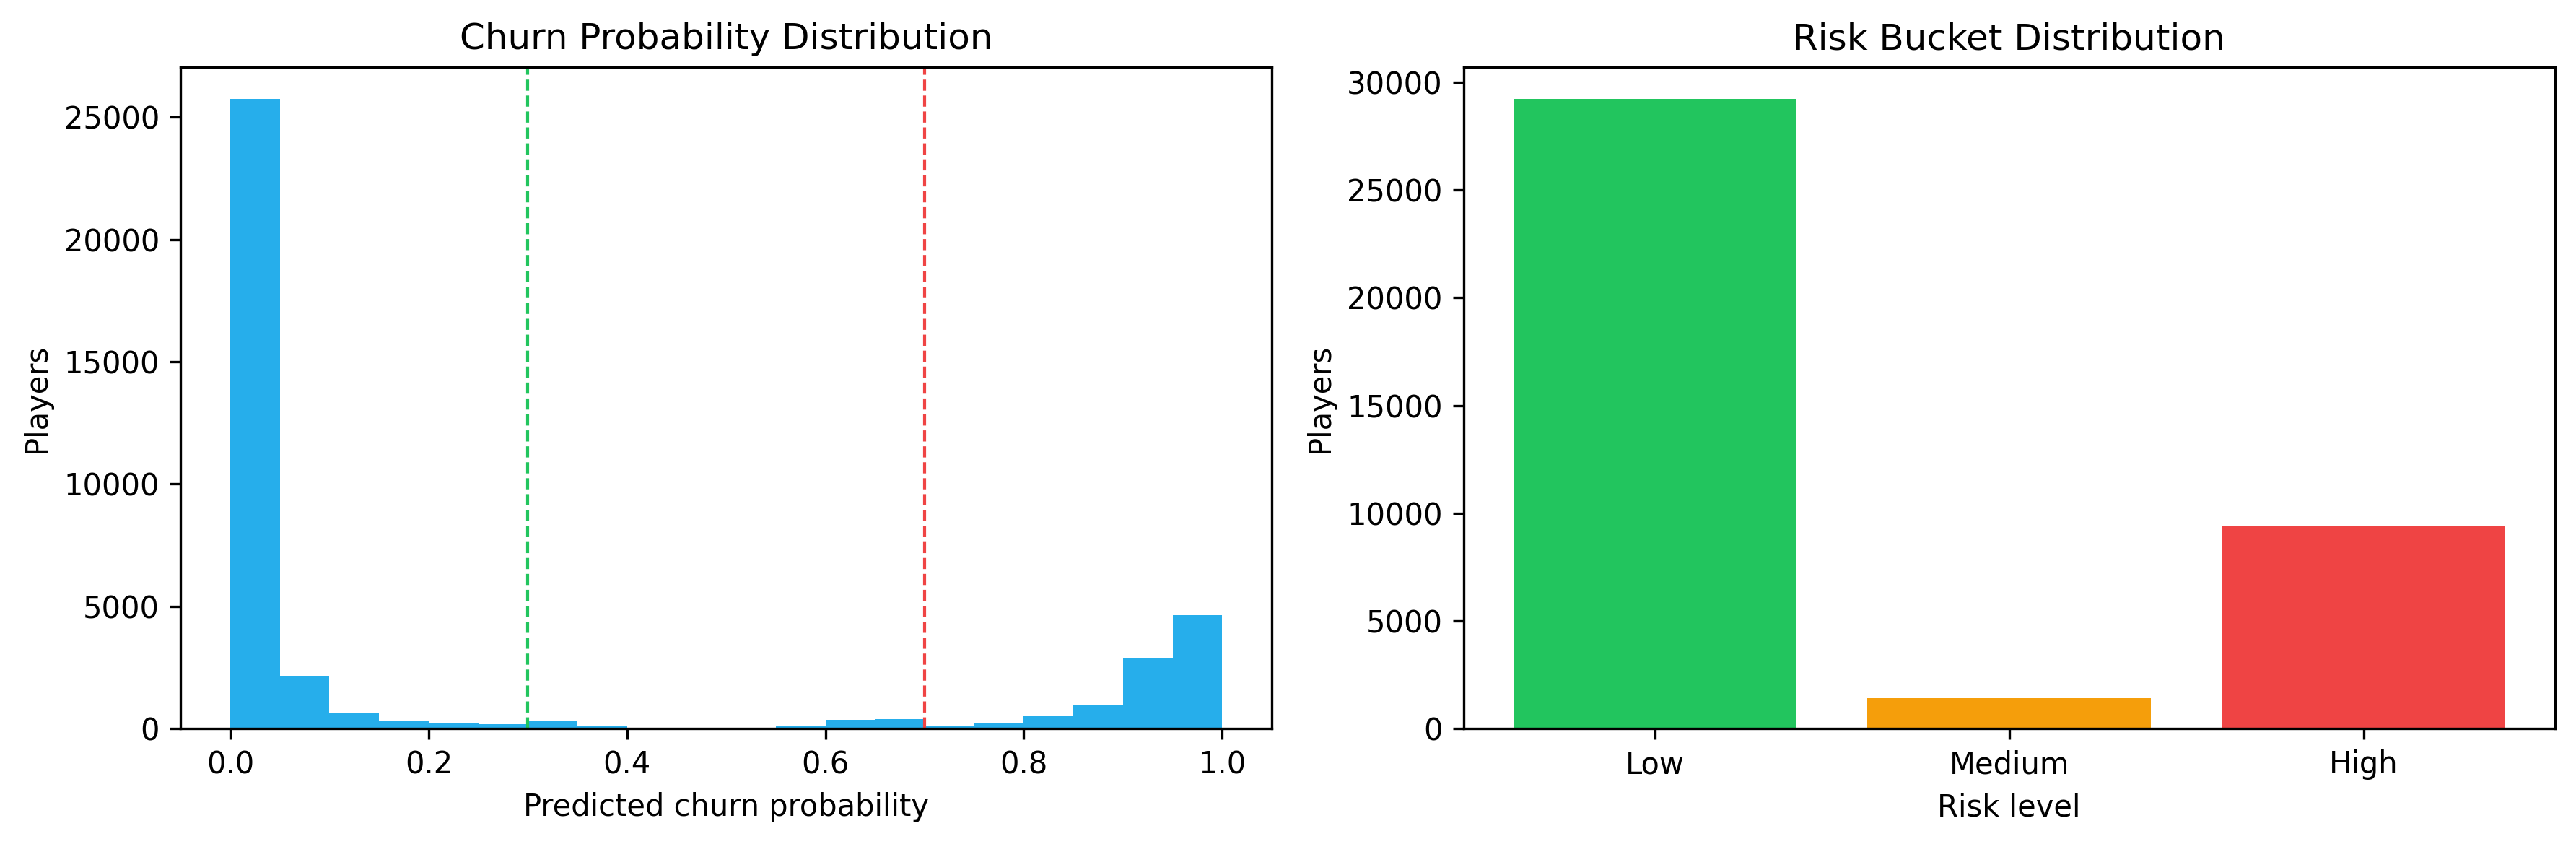
\includegraphics[width=0.45\textwidth]{figures/rf_risk_distribution.png}
\caption{Random Forest churn-probability and risk-bucket distribution.}
\label{fig:rf_risk_distribution}
\end{figure}

\section{Discussion}
Random Forest achieved the best overall performance, with strong balance across precision and recall and the highest F1 and ROC-AUC scores. Logistic Regression produced high recall but lower precision, indicating more false positives. Decision Tree performed competitively but below Random Forest on all major metrics. Limitations include dependence on a single dataset and binary mapping from multi-class engagement labels; future work can include cross-validation, hyperparameter tuning, and temporal validation.

\section{Conclusion}
This project delivers a practical churn prediction framework with:
\begin{itemize}
    \item Unified multi-model training
    \item Standardized evaluation and confusion matrix analysis
    \item Feature-importance-based driver interpretation
    \item Risk segmentation and probability visual analytics
    \item Single-player prediction with UI risk badge rendering
\end{itemize}
The system is suitable for rapid experimentation and retention-focused decision support in gaming analytics.

\bibliographystyle{IEEEtranN}
\bibliography{references}

\appendix
\section{GitHub Repository Information}

\subsection{Repository Link}
\begin{center}
\textbf{\url{https://github.com/atharvgit2005/player_churn_prediction}}
\end{center}

\subsection{Repository Structure}
\begin{lstlisting}[language=bash,caption={Current project structure}]
player_churn_prediction/
|- app.py
|- requirements.txt
|- figures/
|  |- rf_confusion_matrix.png
|  |- rf_risk_distribution.png
\end{lstlisting}

\subsection{Description of Key Components}
\begin{itemize}
    \item \textbf{app.py}: Streamlit application with preprocessing, training, evaluation, visualization, and inference utilities.
    \item \textbf{requirements.txt}: Python dependencies for reproducible deployment.
    \item \textbf{figures/}: Exported evaluation artifacts used in this report.
\end{itemize}

\end{document}
